% presentation
\documentclass{beamer}

% \usetheme{Boadilla}
\usetheme{CambridgeUS}
\usecolortheme{dolphin}

% rus lang
\usepackage[main=russian,english]{babel}

% insert images
\usepackage{wrapfig}
\usepackage{graphicx}
\graphicspath{{./img/}, {../../plots/}}

% math
\usepackage{amsmath}
\usepackage{mathtools}
\usefonttheme[onlymath]{serif}
\newtheorem{rustheorem}{Теорема}

\newcommand{\at}[2][]{#1|_{#2}}
\newcommand{\eps}{\varepsilon}
\renewcommand{\Phi}{\varPhi}
\newcommand{\dd}[2]{\frac{\partial #1}{\partial #2}}

\DeclareMathOperator*{\argmin}{argmin}
\DeclareMathOperator{\sign}{sign}
\DeclareMathOperator{\K}{K}
\DeclareMathOperator{\R}{\mathbb{R}}
\DeclareMathOperator{\X}{\mathbb{X}}
\DeclareMathOperator{\Y}{\mathbb{Y}}
\DeclareMathOperator{\E}{\mathbb{E}}
\DeclareMathOperator{\V}{\mathbb{V}}

% algorithms
\usepackage[linesnumbered,ruled,vlined]{algorithm2e}
\SetKwInput{KwInput}{Input}
\SetKwInput{KwOutput}{Output}
% \SetKwFor{For}{for (}{) $\lbrace$}{$\rbrace$}

\title[Кластеризация]{Лекция 8. Кластеризация}
\subtitle{Основы интеллектуального анализа данных}
\author{Полузёров Т. Д.}
\institute{БГУ ФПМИ}
\date{}

\begin{document}
	
	\begin{frame}
		\titlepage
	\end{frame}
	
	
	\begin{center}
		\frametitle{Структура лекции}
		\tableofcontents
	\end{center}
	
	\section{Постановка задачи}

	\begin{frame}
        \frametitle{Постановка задачи}

		\textbf{Дано}:

		$\X$ --- пространтсов объектов

		$X = \{x_1, \dots, x_{\ell}\}$ --- обучающая выборка

		$\rho : \X \times \X \rightarrow [0, +\infty]$ --- функция расстояния между объектами

		\vspace{15pt}

		\textbf{Необходимо}:

		Определить множество кластеров $\Y$ и построить алгоритм $a : \X \rightarrow \Y$
		так, чтобы:

		\begin{itemize}
			\item каждый кластер состоял из близких объектов
			\item объекты разных кластеров были сущетсвенно различны
		\end{itemize}

		\vspace{15pt}

		Это задача \textbf{кластеризации} --- частный случай задач обучения без учителя.
    \end{frame}

    
	\begin{frame}
		\frametitle{Некорректность задачи кластеризации}
		Особенности задачи:
		\begin{itemize}
			\item точной постановки задачи нет
			\item непонятно как выбрать меру качества кластеризации
			\item априорно неизвестно число кластеров
			\item результат сильно зависит от меры расстояния $\rho$
		\end{itemize}

		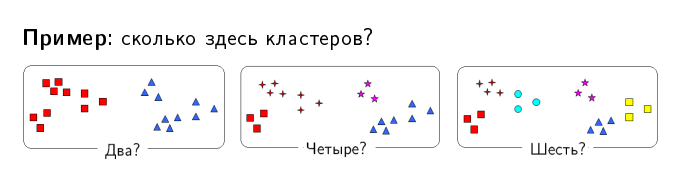
\includegraphics[width=1\textwidth]{img/unk_num_clusters.png}
	\end{frame}

	\begin{frame}
		\frametitle{Цели кластеризации}

		\begin{itemize}
			\item \textbf{Упростить обработку данных},

			разбить все множество $X$ на группы схожих объектов,
			чтобы работать с каждой группой отдельно
			\item \textbf{Сократить объем данных},

			оставить по одному представителю от группы
			\item \textbf{Выделить нетипичные объекты},
			
			которые не относятся ни к одному из кластеров
			\item \textbf{Построить иерархию множества объектов}
		\end{itemize}
	\end{frame}

	\subsection{Типы кластерных структур}

	\begin{frame}
		\frametitle{Типы кластерных структур}

		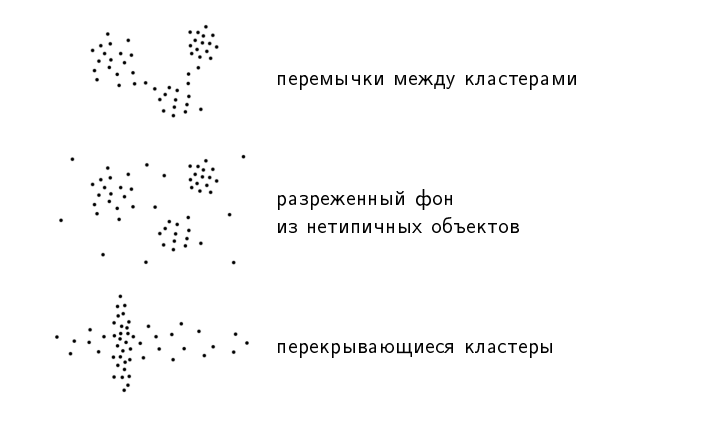
\includegraphics[width=1\textwidth]{img/struct_1.png}

	\end{frame}

	\begin{frame}
		\frametitle{Типы кластерных структур}

		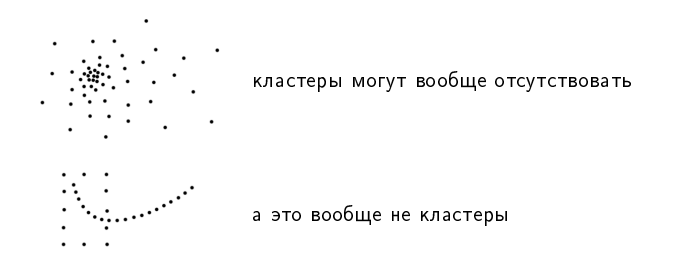
\includegraphics[width=1\textwidth]{img/struct_2.png}

		\begin{itemize}
			\item  кластеры определяются субъективно
			\item каждый метод кластеризации имеет свои ограничения
			и способен работать только на некоторых типах кластеров
		\end{itemize}

	\end{frame}

	\subsection{Меры качества}

	\begin{frame}
		\frametitle{Метрическое пространство}

		Пусть известны только расстояния между оьъектами.

		$a_i = a(x_i)$ --- метка кластера объекта $x_i$

		\begin{itemize}
			\item Среднее внутрикластерное расстояния
			\[
				F_0 = \frac{\sum_{i < j}[a_i = a_j] \rho(x_i, x_j)}
				{\sum_{i < j}[a_i = a_j]} \rightarrow \min
			\]
			\item Среднее межкластерное расстояние
			\[
				F_1 = \frac{\sum_{i < j}[a_i \ne a_j] \rho(x_i, x_j)}
				{\sum_{i < j}[a_i \ne a_j]} \rightarrow \max
			\]
			\item Их отношение
			\[
				\frac{F_0}{F_1} \rightarrow \min
			\]
		\end{itemize}
	\end{frame}

	\begin{frame}
		\frametitle{Векторное пространство}

		Если объекты задаются вектором $x_i \in \R^n$

		\begin{itemize}
			\item Сумма средних внутрикластерных расстояний
			\[
				\Phi_0 = \sum_{a \in \Y} \frac{1}{|X_a|} \sum_{i: a_i = a}
				\rho(x_i, \mu_a) \rightarrow \min
			\]
			где $X_a = \{x_i \in X | a_i = a\}$ --- кластер $a$,
			$\mu_a$ --- центр кластера $a$

			\item Сумма межкластерных расстояний
			\[
				\Phi_1 = \sum_{a, b \in \Y} \rho(\mu_a, \mu_b) \rightarrow \max
			\]

			\item отношение
			\[
				\frac{\Phi_0}{\Phi_1} \rightarrow \min
			\]
		\end{itemize}
	\end{frame}

	\section{K-means}

	\begin{frame}
		\frametitle{Алгоритм: K-средник (K-means) }

		\begin{algorithm}[H]
			\caption{K-means}

			\KwInput{
				$X^{\ell}$, 
				$K$
			}
			\KwOutput{центры кластеров $\mu_a, a = 1, \dots, K$}

			случайно инициализировать $\mu_a, a = 1, \dots, \K$

			\While{не перестанут изменяться $\mu_a$}{
				
				отнести каждый $x_i$ к ближайшему центру
					\[
						a_i := \arg \min_{a \in \Y} || x_i - \mu_a||
					\]

				вычислить новые положения центров
					\[
						\mu_a := \frac{\sum_{i=1}^{\ell} [a_i = a] x_i}
						{\sum_{i=1}^{\ell} [a_i][a]}, a \in \Y
					\]
			}
		\end{algorithm}
	\end{frame}

	\begin{frame}
		\frametitle{Неудачные примеры K-means}

		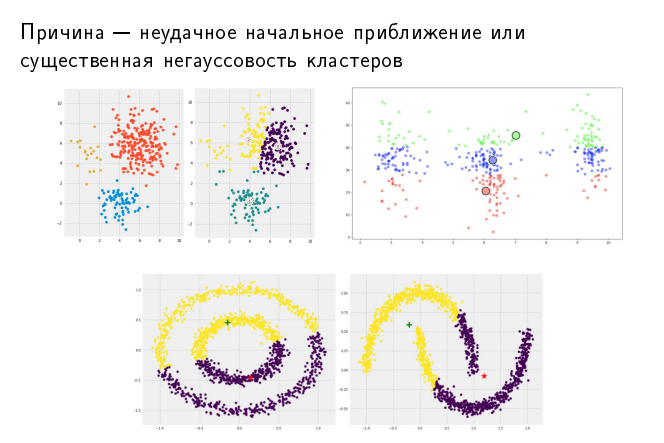
\includegraphics[width=1\textwidth]{img/kmeans_bad.png}
	\end{frame}
	
	\section{DBSCAN}

	\begin{frame}
		\frametitle{Алгоритм: DBSCAN
		
		Density-Based Spatian Clustering of Applications with Noise}

		Зафиксируем 2 параметра:
		\begin{itemize}
			\item $\eps$ --- размер окрестности
			\item $m$ --- параметр плотности
		\end{itemize}

		$\eps$-окресность точки $x \in U$ 
		есть $U_{\eps}(x) = \{u \in U : \rho(x, u) \le \eps\}$ 
		
		\vspace{15pt}

		3 типа объектов:
		\begin{itemize}
			\item \textbf{корневой} --- имеет плотную окрестность, $|U_{\eps}| \ge m$
			\item \textbf{граничный} --- не корневой, но в окрестности корневого
			\item \textbf{шумовой} --- все остальные
		\end{itemize}
	\end{frame}

	\begin{frame}
		\frametitle{Типы точек}

		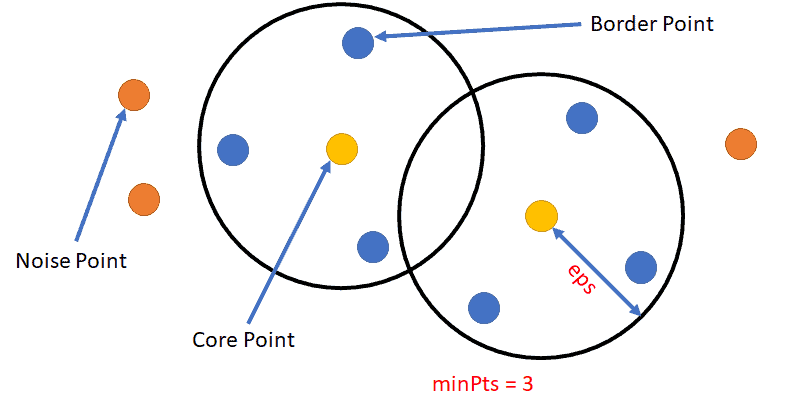
\includegraphics[width=1\textwidth]{img/dbscan_points.png}
	\end{frame}

	\begin{frame}
		\frametitle{}
		
		\begin{algorithm}[H]

			\caption{DBSCAN}
			
			\KwInput{
				$X^{\ell}$, 
				$\eps$,
				$m$
			}
			\KwOutput{разбиение на кластеры, определение шумовых объектов}

			$U := X$ --- неразмеченные объектов
			$k := 0$ --- номер кластера

			
			\While{$U \ne \emptyset$}{
				
				взять случайный объект $x \in U$
				
				\If{$U_{\eps}(x) < m$}
				{
					пометить шумовой
				}
				\Else
				{
					$k++$ --- создать новый кластер,
					$K := U_{\eps}(x)$

					\While{$K \ne \emptyset$}
					{
						$x^{'} := K.pop()$ --- не помеченый и не шумовой

						\If{$U_{\eps}(x^{'}) \ge m$}
						{
							$K.add(U_{\eps}(x^{'}))$ и пометить $x^{'}$ как корневой
						}
						\Else
						{
							пометить $x^{'}$ как граничный
						}
					}
				}
				
			
			}
		\end{algorithm}
	\end{frame}

	\begin{frame}
		\frametitle{K-means vs DBSCAN}

		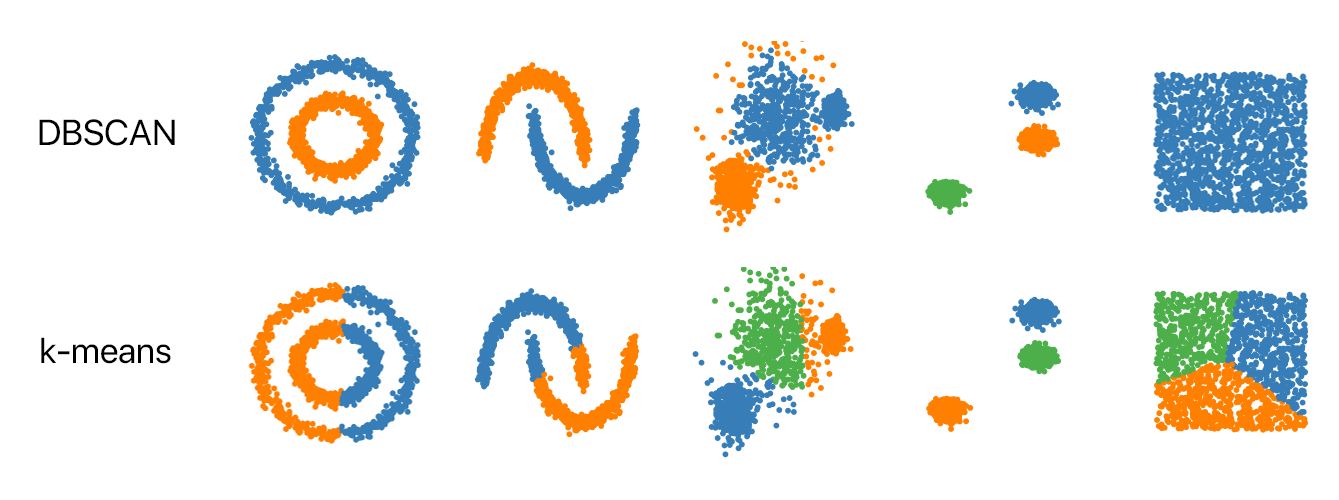
\includegraphics[width=1\textwidth]{img/kmean_vs_dbscan.png}
	\end{frame}

	\section{Иерархическая кластеризация}

	\begin{frame}

		$R_{UV}$ --- мера расстояния между кластерами $U$ и $V$

		\begin{algorithm}[H]
			\caption{Иерархическая кластеризация}

			$С_1 := \{\{x_1\}, \dots, \{x_{\ell}\}\}$
			
			\For{$t = 2, \dots, \ell$}{
				найти в $C_{t-1}$ пару кластеров $(U, V)$  с минимальным $R_{UV}$

				слить их в один кластер

				$W := U \cup V$

				$C_t := C_{t-1} \cup \{W\} \setminus \{U, V\}$

			}
		\end{algorithm}	
	\end{frame}

	\begin{frame}
		\frametitle{Дендрограмма}

		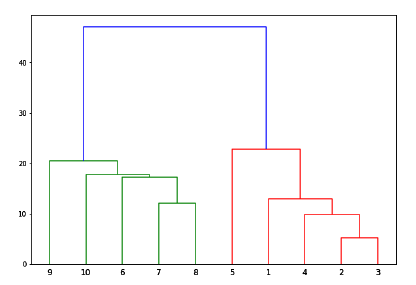
\includegraphics[width=1\textwidth]{img/ierarh.png}
	\end{frame}

	\begin{frame}
		\frametitle{Итого}

		\begin{itemize}
			\item Кластеризация --- частный случай обучения без учителя
			\item Ключевая концепция --- близость похожих объектов 
			\item Изначально задача поставлена некорректно
			\item Каждый алгоритм подходит для определенного типа кластеровной структуры
		\end{itemize}
	\end{frame}
\end{document}
